\section{Component Types}
With the introduction of software components, the question of their substitutability arises. A component is not only defined by its provided interfaces, but also by the interfaces required from the environment. So, the constraints for replacing a component are more complex. The UML 2.0 superstructure addresses this issue only curtly:

\begin{quote}
``As such a component serves as a \emph{type}, whose conformance is defined by these provided and required interfaces. One component may therefore be substituted by another only if the two are type conformant.''
%TODO add reference: UML Superstructure p.150
\end{quote}

Here \emph{component types} and \emph{conformance} between components and types are mentioned. However, both concepts are not further clarified. We need a clear and useful definition of both terms to provide a component meta model that allows (a)  interoperability and substitutability checks of components and (b) enables the prediction of Quality of Service attributes of a component in a certain context.

In the following, we develop a more detailed approach to component types that allows different notions of substitutability. We also clarify the conformance of a component to a type. We introduce these concepts using the architecture of a web server shown in figure \ref{fig:WebserverComponents} and give a formal definition of the terms in the end of this section.

\begin{figure}[htbp]
\centering
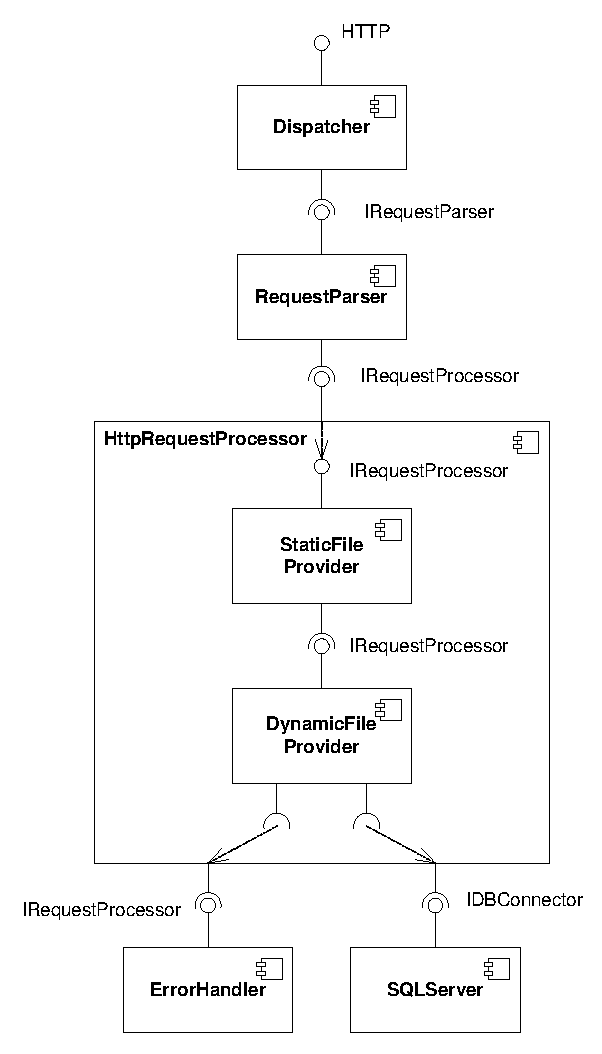
\includegraphics[width=3.3in]{example/WebserverComponents}
\caption{Component architecture of a web server.}
\label{fig:WebserverComponents}
\end{figure}

The main part of the web server is realised by the three components dispatcher, RequestParser, and HttpRequestProcessor. The Dispatcher listens on a set of incoming connections and spawns a new tread for each incoming HTTP request, which activates the RequestParser. The parser analyses the request and passes the result to the HttpRequestProcessor. The request processor is organised as a Chain of Responsability \cite{gamma1995a}. Each of its subcomponents checks whether it can handle the incoming request. If so, it returns the result, otherwise it passes the request to the next component in the chain. The ErrorHandler represents the end of the chain and returns an error message, if the request could not be handled by any of the components. Additionally, the SQLServer is required to create dynamic HTML pages.

Looking at the architecture of the web server, we can identify at least two different types of components, which appear several times in the architecture. The components \texttt{StaticFileProvider} and \texttt{HttpRequestProcessor} provide and require the IRequestProcessor interface. The type of both components is shown in figure \ref{fig:RequestProcessorType}.

\begin{figure}[htbp]
\centering
\includegraphics[scale=1.0]{example/RequestProcessorType}
\caption{Another component type used in the web server.}
\label{fig:RequestProcessorType}
\end{figure}

The components HttpRequestProcessor and DynamicFileProvide additionally require the IDBConnector interface to create the dynamic content of the pages. The type of these components is shown in figure \ref{fig:DynamicRequestProcessorType}.

\begin{figure}[htbp]
\centering
\includegraphics[scale=1.0]{example/DynamicRequestProcessorType}
\caption{A component type used at different points in the web server.}
\label{fig:DynamicRequestProcessorType}
\end{figure}

The types shown in figure \ref{fig:RequestProcessorType} and \ref{fig:DynamicRequestProcessorType} describe the complete functionality provided and required by all components of one of these types. A component conforms to a type, if it offers at least the functionality specified in the provided interfaces. It can have additional provided interfaces, which are not included in the type. So, a component must offer the IRequestProcessor interface to conform to one of the types in figure \ref{fig:RequestProcessorType} or \ref{fig:DynamicRequestProcessorType}. Furthermore, a component can only use services that are specified in the required interfaces of the type. For example, the DynamicFileProvider does not conform to the RequestProcessorType, since it uses the IDBConnector interface. Note that a component does not have to use all required interfaces of its type. So, all components that conform to the RequestProcessorType also conform to the DynamicRequestProcessorType, since they do not require the IDBConnectorInterface. 

This understanding of conformance between components and types allows us to define substitutability of components.--TODO: How?-- However, in many cases we are not only interested in a complete substitutability that includes provided and required interfaces, but in a substitutability with respect to the provided interfaces only. This is the case if we replace a component and do not care for its required interfaces or if we want to compare only the functionality offered by a component. 



\begin{figure}[htbp]
\centering
\includegraphics[scale=1.0]{example/ProvidesType}
\caption{Provides-type of the RequestProcessorType and DynamicRequestProcessorType.}
\label{fig:ProvidesType}
\end{figure}

So, we want to allow conformance with respect to provided interfaces only. Therefore, we introduce a \emph{provides-type} which only describes provided interfaces. The provides-type of the RequestProcessortType and the DynamicRequestProcessorType is shown in figure \ref{fig:ProvidesType}. --TODO: Picture with hierarchy instead--

Contravariance, required and provided interfaces as contracts

This is not the only Type that is used in the component model of the web server.

So, some components provide the same interfaces, but require different services to complete their task.
Distinguish between Provided and Complete types. Both have their advantages. They are defined by substitutability. 

The development process of a component is not fixed to both types of a component, but is an evolutionary process.
During Software architecture design, there is no clear border between both types.

The stepwise completion of a component specification leads to different interpretations of required interfaces.
-	can be used, but there can be more (provided type interpretation)
-	can only be used (complete type)
-	has to be used in a predefined fashion (not considered in our case, example: information has to be stored in a database, so the interface of the database must be used.

Conformance between Provided and Complete Types.
